\chapter{Results}
\thispagestyle{empty}

\section{Expectation}

\section{Dictionay elements}
\begin{figure}
\centering
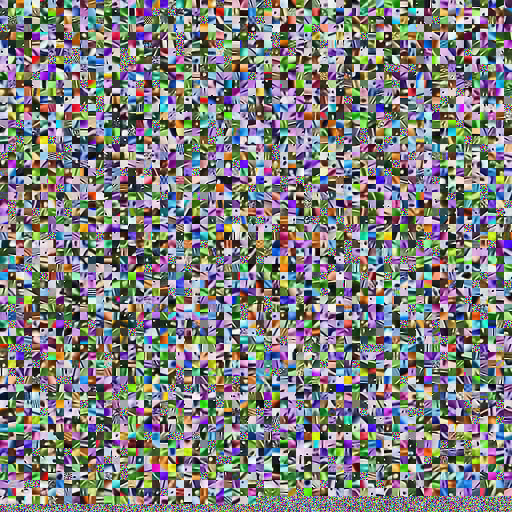
\includegraphics[width = 0.66\textwidth]{images/8_4000_10000_10_lasso.png} 
\caption{8x8 LARS-lasso with 4000 elements}
\label{fig:8_4000_lasso}
\end{figure}

\begin{figure}
\centering

\includegraphics[width = 0.33\textwidth]{images/gradient.png} 
\caption{gradient}
\label{fig:gradient}
\end{figure}

\begin{figure}
\centering

\includegraphics[width = 0.33\textwidth]{images/checkerboard.png}
\caption{checkerboard}
\label{fig:checkerboard}
\end{figure}


\begin{figure}
\centering

\includegraphics[width = 0.33\textwidth]{images/spot.png} 
\caption{spot}
\label{fig:spot}
\end{figure}


\begin{figure}
\centering

\includegraphics[width = 0.33\textwidth]{images/edges.png}
\caption{edge}
\label{fig:edge}
\end{figure}

\begin{figure}
\centering
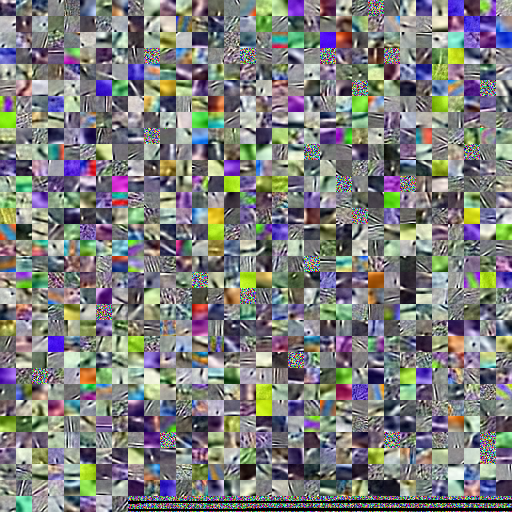
\includegraphics[width = 0.66\textwidth]{images/16_1000_1000_10_lasso.png}
\caption{16x16 LARS-lasso with 1000 elements}
\label{fig:16_1000_lasso}
\end{figure}

\begin{figure}
\centering

\includegraphics[width = 0.33\textwidth]{images/wavelet.png}
\caption{wavelets}
\label{fig:wavelets}
\end{figure}

\section{Quality}
\subsection*{trained vs. analytical base}
\subsection*{Compression ratio}
\subsection*{Dictionary size}
Setup:
  initialize: random pixels, radom samples 
  dict size: 256, 1000, 4000, 8000
  coeffs: 5, 10, 20

\section{Compression}







